%%
%% 2019 07 04 Ph. G. Freimann
%% 2020 Systematik verbessert
%%

\section{Lineare Funktionen}\index{Funktion!lineare}
\index{affin-lineare Funktionen}\label{lineare_funktionen}
\sectuntertitel{$f: \mathbb{R} \rightarrow \mathbb{R}$}
%%%%%%%%%%%%%%%%%%%%%%%%%%%%%%%%%%%%%%%%%%%%%%%%%%%%%%%%%%%%%%%%%%%%%%%%%%%%%%%%%
\subsection*{Lernziele}

\begin{itemize}
\item Begriff «Lineare Funktion»
\item Darstellungen (Wertetabelle, Funktionsgleichung, Graph)
\item Charakteristische Punkte\index{Punkt!charakteristischer}
  \begin{itemize}
  \item
    y-Achsenabschnitt (Ordinatenabschnitt)
  \item Nullstelle
  \end{itemize}
\item Steigung
\TALS{\item Taschenrechner: Darstellung von Graphen}
\end{itemize}

Theorie:
\TALS{(\cite{frommenwiler17alg} S.170 (Kap. 3.3))}
\GESO{(\cite{marthaler21}       S.237 (Kap. 14))}
\newpage

\subsection{Einstiegsbeispiel Taxiunternehmen}
Taxiunternehmen «A» hat eine Grundgebühr von CHF 10.- und kostet
danach CHF 0.60 pro gefahrenen Kilometer.

Taxiunternehmen «B» hat eine Grundgebühr von CHF 6.- und kostet
danach CHF 0.90 pro gefahrenen Kilometer.

Ab bzw. bis wo lohnt sich das Unternehmen «A» bzw. «B»?

  Zeichnen Sie ein Koordinatensystem. $x$-Achse = km; $y$-Achse = CHF.
  (Einteilung je ca. 20 Einheiten im 1. Quadranten.

\TNTeop{%%
    \bbwCenterGraphic{14cm}{allg/funktionen/img/Taxiunternehmen.png}

  Ablesen bei ca. 13.33 km.

  Rechnerisch:

  $$A: 10\textrm{[CHF]}
  +x\textrm{[km]}\cdot{} 0.60 \left[\frac{\textrm{CHF}}{\textrm{km}}\right] $$
  $$B: 6 +x \cdot{} 0.90$$
  Gleichstand bei:
  $$10+0.6x = 6+0.9x$$
  Lösung:
  $$x = 13.\overline{3} \textrm{km}$$
}%% END TNT

%%%%%%%%%%%%%%%%%%%%%%%%%%%%%%%%%%%%%%%%%%%%

\subsection{Beispiel einer linearen Funktion}
Zeichnen Sie den Graphen der Funktion $f: y= -0.5x + 1$ in ein rechtwinkliges Koordinatensystem:

\bbwGraph{-4}{4}{-1}{4}{
  \TRAINER{\bbwFunc{-0.5*\x + 1}{-3:3}}
}%% end bbwGraph

%%\noTRAINER{\bbwGraph{-4}{4}{-1}{4}{}}
%%\TRAINER{\bbwFunction{-4}{4}{-1}{4}{-0.5*\x + 1}{-3:3}}

\GESO{
  \paragraph{Punkte mit dem Taschenrechner}: Mit der ``TABLE''-Funktion auf Ihrem Taschenrechner lassen sich Wertetabellen ganz einfach erstellen.
  Füllen Sie eine Wertetabelle zur Funktion $f: y=\frac{3}{4}x  - 1.5$ aus und zeichnen Sie die Gerade ein ein rechtwinkliges Koordinatensystem:

  \begin{tabular}{l|c|c|c|c|c|c|c}
    $x$ & -2 & -1 & 0 & 1 & 2 & 3 \\
    $y$ & \LoesungsRaum{-3}   & \LoesungsRaum{-2.25}   & \LoesungsRaum{-1.5}  & \LoesungsRaum{-0.75}  & \LoesungsRaum{0}  &  \LoesungsRaum{0.75} \\
  \end{tabular}


  \bbwGraph{-4}{4}{-4}{2}{
    \TRAINER{\bbwFunc{0.75*\x - 1.5}{-2.5:3.5}}
  }%% END bbw Graph
  %%\noTRAINER{\bbwGraph{-4}{4}{-4}{2}{}}
  %%\TRAINER{\bbwFunction{-4}{4}{-4}{2}{0.75*\x - 1.5}{-2.5:3.5}}
  
   \newpage
}

\subsection{Definition der linearen Funktion}\index{Lineare Funktion!Definition}
\begin{definition}{}{}

  Eine Funktion $f: x\mapsto f(x)$ von $\mathbb{R}$ nach $\mathbb{R}$ heißt
\textbf{linear}\index{lineare Funktion}, wenn sie in der Grundform
$$f(x) = y=a\cdot{}x + b$$
mit $a$ und $b$ in $\mathbb{R}$ dargestellt werden kann.
\end{definition}


Beispiele:

\vspace{3mm}
\hrule
\vspace{3mm}

$$f(x) = y = \LoesungsRaumLang{4x + 1.5}$$
(Hier ist $a=\LoesungsRaum{4}$ und $b=\LoesungsRaum{1.5}$.)

\vspace{3mm}
\hrule
\vspace{3mm}

$$f(x) = y = \LoesungsRaumLang{-x}$$
(Hier ist $a=\LoesungsRaum{-1}$ und $b=\LoesungsRaum{0}$.)

Ist $b=0$, so sprechen wir auch von einer Proportionalität.

\vspace{3mm}
\hrule
\vspace{3mm}

$$f(x) = y = \LoesungsRaumLang{-0.6}$$
(Hier ist $a=\LoesungsRaum{0}$ und $b=\LoesungsRaum{-0.6}$.)

Ist $a=0$, so sprechen wir auch von der konstanten Funktion.

\vspace{3mm}
\hrule

\GESO{\subsection*{Aufgaben}}
\GESOAadBMTA{250}{6. a) b)}
\newpage



\subsection{Charakteristische Punkte}\index{Punkte!charakteristische}\index{charakteristische Punkte}
Jede lineare\footnote{
  Die linearen Funktionen werden eingeteilt in die \textbf{Proportionalitäten} für $b=0$ und in die \textbf{affinen Abbildungen} für $b\ne{}0$.} Funktion schneidet irgendwo die beiden\footnote{Ausnahme: Konstante. Eine Konstante $y=b$ schneidet nur die $y$-Achse. Der Spezialfall $y=0$ \textbf{ist} die $x$-Achse.} Achsen. Zeichnen Sie die Funktion $f: y=\frac{1}{2}x  +3$ und notieren Sie die Punkte, wo die x- bzw. die y-Achse von unserer Geraden geschnitten wird:

\vspace{1cm}

Wertetabelle:

\begin{tabular}{c|p{2cm}|p{2cm}|p{2cm}|p{2cm}|p{2cm}|p{2cm}}
   x  & 0 & 1 & 2 & 4 & -4 & \TRAINER{-6}\\\hline
   y  & \TRAINER{3} & \TRAINER{3.5} & \TRAINER{4}& \TRAINER{5}&\TRAINER{1}&0\\%%
\end{tabular}


\bbwGraph{-7}{7}{-2}{5}{}
\newpage

\subsubsection{$y$-Achsenabschnitt}\index{$y$-Achsenabschnitt}\index{Achsenabschnitt!y-}\index{Ordinatenabschnitt}
\begin{definition}{$y$-Achsenabschnitt}{}
  Der Parameter $b$ wird $y$-Achsenabschnitt
(oder Ordinatenabschnitt\index{Ordinatenabschnitt}\footnote{Die
    $y$-Koordinate eines Punktes wird auch
    \textbf{Ordinate}\index{Ordinate} und die $x$-Koordinate wird auch
    \textbf{Abszisse}\index{Abszisse}  genannt.}) genannt.
  
Dieser gibt an, in welcher «Höhe» die Gerade die y-Achse schneidet.
\end{definition}

Wir erhalten den $y$-Achsenabschnitt, indem wir das Funktionsargument $x$
gleich Null (0) setzen: $x=0$.

Somit wird
$$y=ax+b$$
$$y=a\cdot{}0+b$$
$$y=b$$
Was uns zeigt, dass der  Punkt $P=(0|b)$ der Geraden immer auf der $y$-Achse liegt.

\newpage

\subsubsection{Nullstelle}\index{Nullstelle}
Wo schneidet der Funktionsgraph die $x$-Achse?

Dazu setzen wir $f(x)=y=0$, und lesen wir den Schnittpunkt in obiger Grafik etwa bei $x=-6$ ab.

\begin{definition}{Nullstelle}{}
  Eine \textbf{Nullstelle} ist gibt an, an welcher Stelle der Funktionsgraph die $x$-Achse schneidet.
\end{definition}


Die Nullstelle einer linearen Funktion in ihrer Grundform ist die Lösung der entsprechenden linearen Gleichung (mit
$y$=0) in ihrer Grundform. Nämlich:

a) Lineare Gleichung $ax+b=0$

Gesucht \textbf{Lösung} $x$:

$$x = \frac{-b}{a}  $$

b) Lineare Funktion $f: y=ax+b$

Gesucht \textbf{Nullstelle} $x_0$ bei $y_0=0$. Die Gerade schneidet
die $x$-Achse in der Nullstelle $x_0$ der Geraden. Somit ist der
Schnittpunkt wie folgt gegeben:

$$N(x_0|y_0) = N\left( \frac{-b}{a}\,\, \bigg|\,\, 0 \right) $$



\newpage


\subsubsection{Steigung}\index{Steigung|textbf}
  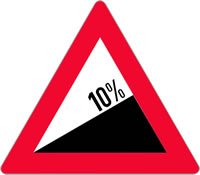
\includegraphics[width=4.5cm]{tals/trig1/img/starkeSteigung.jpg}

Der Parameter $a$ wird Steigung der Geraden genannt. Dies entspricht
dem $y$-Anstieg\footnote{Bei negativem $a$ sprechen wir von «Gefälle»,
  Abstieg, Neigung, Senkung, ...} der Geraden pro Einheit in $x$-Richtung ($e_x$):


%% Steigungsgraph: Eins nach rechts -> a noch oben (oder -a nach unten)
\bbwGraph{-4}{4}{-3}{4}{
	\draw[thick] (-4,-2.5) -- (4, 3.5);
	\draw[thick,color=blue] (1, 1.25) -- (2  , 1.25);
	\draw[thick,color=blue] (1, 1.25) -- (1.5, 1.25) node[anchor=north]{${\color{blue}1}$};
	\draw[thick,color=red ] (2, 1.25) -- (2, 2   );
	\draw[thick,color=red ] (2, 1.25) -- (2, 1.625   ) node[anchor=west ]{${\color{red}a}$ };
}

\newpage


Steigt die Gerade in $x$-Richtung an, so ist ${\color{blue}a}$ positiv (${\color{blue}a>0}$);
fällt die Gerade in $x$-Richtung ab, so ist ${\color{red}a}$ negativ (${\color{red}a<0}$).

%% Steigungsgraph: Eins nach rechts -> a noch oben (oder -a nach unten)
\bbwGraph{-4}{4}{-3}{4}{
	\draw[thick,color=blue] (-4, -1) -- (4  , 3);
	\draw[thick,color=blue] (4, 3) node[anchor=north]{${\color{blue}+}$};
	\draw[thick,color=red ] (-3.5, 2) -> (4, -2);
	\draw[thick,color=red ] (4, -2) node[anchor=west ]{${\color{red}-}$ };
}

Die Steigung $a$ kann aus \textbf{jedem} Steigungsdreieck berechnet werden,
wozu einfach zwei Punkte auf der Geraden zu verwenden sind:

%% Steigungsgraph: Eins nach rechts -> a noch oben (oder -a nach unten)
\bbwGraph{-4}{4}{-3}{4}{
	\draw[thick] (-4,-11/5) -- (4, 13/5);
	\draw[thick,color=blue] (-2, -1) -- (3,-1);
	\draw[thick,color=blue] (1, -1.1) node[anchor=north]{${\color{blue}H}$};
  
	\draw[thick,color=red] (3, -1) -- (3,2);
	\draw[thick,color=red] (3, 1.1) node[anchor=west]{${\color{red}V}$};

  \bbwDot{-2,-1}{black}{north}{}
  \bbwDot{3,2}{black}{north}{}
  \bbwDot{3,-1}{black}{north}{}
}
\newpage

\begin{rezept}{Finden der Geradensteigung}{}
Die Steigung $a$ ist:
$$a=\frac{{\color{red}V}}{{\color{blue}H}}$$
«Vau durch Haa, das gibt das Ahh!»
\end{rezept}

\subsubsection*{Herleitung (optional)}
\TNTeop{
  \bbwCenterGraphic{10cm}{allg/funktionen/img/Steigungsdreieck.png}

 $$\frac{V}H = \frac{\Delta y}{\Delta x} = \frac{y_2-y_1}{x_2-x_1} =
  \frac{f(x_1) - f(x_2)}{x_2-x_1}$$

  $$= \frac{(a\cdot{}x_2 + b) - (a\cdot{}x_1 +b)}{(x_2-x_1)}$$
  $$= \frac{a\cdot{}x_2 + b - a\cdot{}x_1 -b}{(x_2-x_1)}$$
  $$= \frac{a\cdot{}x_2 - a\cdot{}x_1 }{(x_2-x_1)}$$
  $$= \frac{a\cdot{}(x_2 - x_1 )}{(x_2-x_1)}$$
  $$= a$$
}%% END TNT eop

%%%%%%%%%%%%%%%%%%%%%%%%%%%%%%%%%%%%%%%%%


\subsection*{Aufgaben}

\GESO{\olatLinkArbeitsblatt{Lineare Funtkionen}{https://olat.bbw.ch/auth/RepositoryEntry/572162163/CourseNode/102901171745363}{«Steigung, $y$-Achsenabschnitt, Nullstelle}}
\TALS{\TRAINER{... Aufgabenblatt zu TALS SAN (coming soon)....}}

\GESOAadBMTA{250ff}{5. a) (1) und b) (1), 7. a), 8. a) [Ursprungsgerade =
  Gerade durch den Nullpunkt], 10., 23. a) c) e) und optional
  20. (Alkohol im Blut)}

\newpage


\subsection{Referenzaufgaben}\index{Lineare
  Funktion!Referenzaufgaben}\index{Referenzaufgaben zu linearen Funktionen}




\subsubsection{\TALS{Senkrechte und
  }Parallele}\index{Parallele}\TALS{\index{Senkrechte}}\index{Parallele}

\paragraph{Die zwei Parallelen} (Christian Morgenstern)
\begin{verse}
Es gingen zwei Parallelen\\
ins Endlose hinaus,\\
zwei kerzengerade Seelen\\
und aus solidem Haus.

Sie wollten sich nicht schneiden\\
bis an ihr seliges Grab:\\
Das war nun einmal der beiden\\
geheimer Stolz und Stab.

Doch als sie zehn Lichtjahre\\
gewandert neben sich hin,\\
da wards dem einsamen Paare\\
nicht irdisch mehr zu Sinn.

War'n sie noch Parallelen?\\
Sie wußtens selber nicht, ---\\
sie flossen nur wie zwei Seelen\\
zusammen durch ewiges Licht.

Das ewige Licht durchdrang sie,\\
da wurden sie eins in ihm;\\
die Ewigkeit verschlang sie\\
als wie zwei Seraphim.
\end{verse}
\newpage



\paragraph{Parallele:} Skizzieren Sie $f: y=\frac{1}{4}x +3$ und $g:
y=\frac{1}{4}x -1$. Was fällt Ihnen auf?

\bbwGraph{-1}{6}{-2}{5}{}

\TALS{
\paragraph{Senkrechte} Zeichnen Sie eine Senkrechte zur folgenden
Geraden:

\bbwGraph{-1}{6}{-2}{4}{
  \bbwLine{-1,-1.25}{6,0.5}{green}
  \bbwDot{0,-1}{blue}{east}{}
  \bbwDot{4,0}{blue}{north}{}
}
}


\TALS{
\begin{center}
\begin{tabular}{c|c|c}
  Gerade     & Parallele  & Senkrechte \\
  \hline
  $y=ax+b_1$ & $y=ax+b_2$ & $y=-\frac{1}{a}x + b_3$\\
\end{tabular}
\end{center}
}

\GESO{
\begin{center}
\begin{tabular}{c|c}
  Gerade     & Parallele \\
  \hline
  $y=ax+b_1$ & $y=ax+b_2$ \\
\end{tabular}
\end{center}
}

\TALS{
Da es beliebig viele Senkrechte und Parallele zu einer gegebenen
Geraden gibt, kann nur auf die Steigung eine Aussage gemacht
werden. Sowohl $b_2$, wie auch $b_3$ können erst ermittelt werden,
wenn weitere Angaben (wie \zB{} ein weiterer Punkt) vorhanden sind.

Beachten Sie, dass hier $a$ natürlich nicht Null (0) sein darf.
}

\GESO{
Da es beliebig viele Parallele zu einer gegebenen
Geraden gibt, kann nur auf die Steigung eine Aussage gemacht
werden. $b_2$ kann erst ermittelt werden,
wenn weitere Angaben (wie \zB{} ein weiterer Punkt) vorhanden sind.
}


\newpage


\subsubsection{Ein Punkt ist gegeben}\index{Punkt auf Geraden}\index{Gerade!Punkt auf}
Bei vielen Anwendungen ist von der Geraden die Steigung $a$
\textbf{oder} der $y$-Achsenabschnitt $b$ gegeben, aber nicht
beides. Dabei ist meist ein Punkt $P$ (\zB $P=(7|4)$) gegeben, durch
den die Gerade laufen muss.

Gleich zwei Beispiele:

\begin{tabular}{p{8cm}|p{8cm}}
  Steigung gegeben & $y$-Achsenabschnitt gegeben \\
  ${\color{orange}y}=3\cdot{}{\color{blue}x}+b$ & ${\color{orange}y}=a\cdot{}{\color{blue}x}+1.5$\\
  \hline
  Punkt $P=({\color{blue}7}|{\color{orange}4})$ gegeben & Punkt $P=({\color{blue}7}|{\color{orange}4})$ gegeben\\
  \hline
  einsetzen: & einsetzen: \\
  ${\color{orange}4} = 3\cdot{}{\color{blue}7} + b$ & ${\color{orange}4}=a\cdot{}{\color{blue}7} + 1.5$\\
  \hline
  lösen & lösen\\
  $\longrightarrow b=4-21=-17$ & $\longrightarrow a=\frac{4-1.5}{7} =\frac{2.5}{7}=\frac{5}{14} \approx{} 0.357$

  \end{tabular}


\begin{rezept}{Einsetzen}{}
Koordinaten des gegebenen Punktes in die
  Geradengleichung einsetzen, um $a$ bzw. $b$ zu finden!
\end{rezept}

\GESOAadBMTA{252ff}{13. a) d), 14. a) c), 34. a) b) und 35.}

\newpage


\subsubsection{Gerade durch zwei gegebene Punkte}\index{Punkt auf Geraden}\index{Gerade!Punkt auf}
\TALS{Einstiegsaufgaben Frommenwiler: 606. a) c)}

Seien die Punkte $P=(10|6)$ und $Q=(-5|3)$ gegeben.
Gesucht ist die Funktionsgleichung $f: y=ax+b$ (namentlich $a$ und $b$), sodass
der Graph der Funktion $f$ durch beide Punkte führt.


\paragraph{Rezept I: Graphisch}\,

\vspace{1mm}

\TNT{8.4}{\raisebox{2cm}{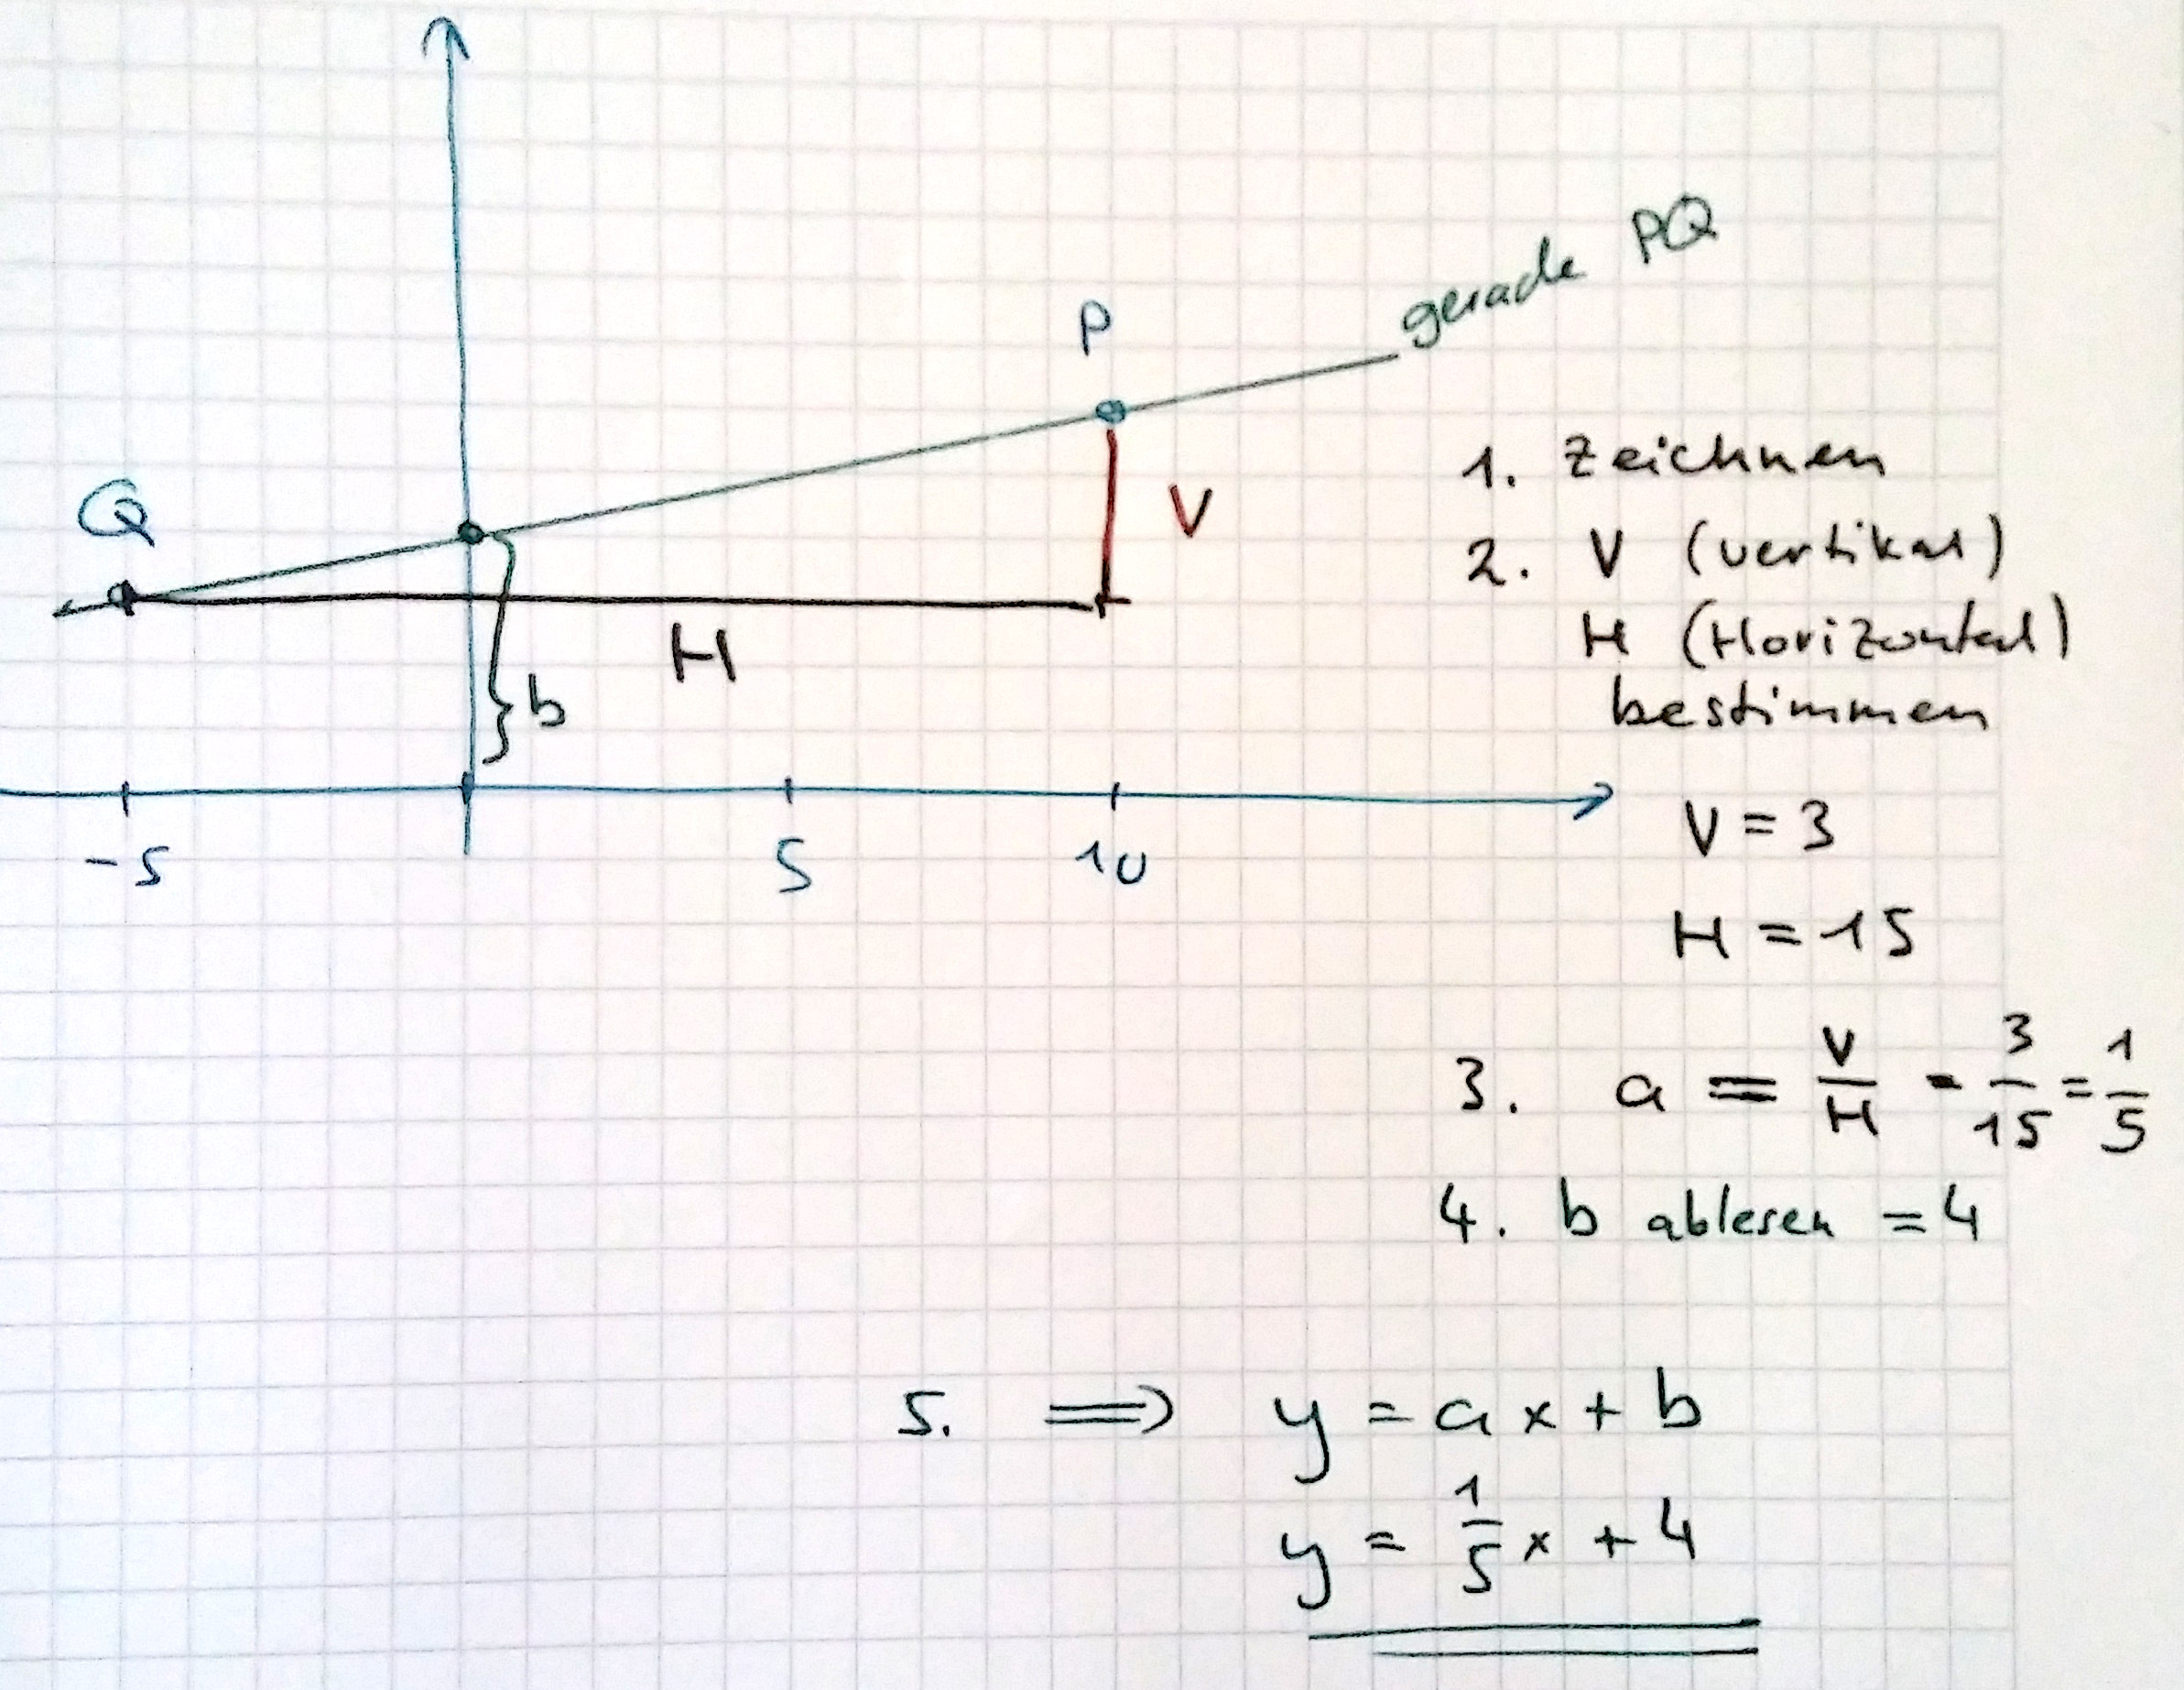
\includegraphics[width=12cm]{allg/funktionen/img/GeradeDurchZweiPunkte.jpg}}}
\newpage


\paragraph{Rezept II: Rechnerisch (algebraisch)}\,

\vspace{1mm}

\begin{rezept}{}{}
Um die Funktionsgleichung $$y=ax+b$$ zu finden,
  werden die $x$- und $y$-Koordinaten der beiden Punkte in die Gleichung eingesetzt und die beiden Gleichungen werden nach $a$ und $b$ aufgelöst. 
\end{rezept}

\TRAINER{

  TAFELText: Um $a$ und $b$ zu finden, setzen wir die $x$- und
  $y$-Koordinaten der beiden Punkte in die Funktionsgleichung ein.}
\noTRAINER{\vspace{12mm}}

Dies ergibt das folgende Gleichungssystem\footnote{Für $P$ gilt: $(x_P|y_P)=(x_P|f(x_P))=(x_P|ax_P+b)$ und somit $y_p =ax_P + b$.}:

\TNT{3.2}{\gleichungZZ%
{6}{a\cdot{}10 + b}%
{3}{a\cdot{}(-5) + b}
\vspace{1cm}
}%% END TNT

Die Subtraktion der beiden Gleichungen ergibt $3 = 15a$, was uns zu $a=\frac{1}{5}$ bringt.

Das $a$ kann auch durch das «Steigungsdreieck» berechnet werden:

$$a = \frac{y_Q-y_P}{x_Q-x_p} = \frac{3 - 6}{-5 - (-10)} = \frac{-3}{-15} = \frac{1}{5}$$

Setzen wir $a=\frac{1}{5}$ in eine der beiden Gleichungen ein, so erhalten wir $b=4$. Die gesuchte Geradengleichung lautet also:

$$f: y=\frac{1}{5}\cdot{}x + 4$$

\TALS{%%
Dies kann auch mit dem Taschenrechner gelöst werden; denn für alle Punkte $P$ auf $f$ gilt ja $P(x|y) = P(x|f(x))$:

$$f(x):=a\cdot{}x + b$$
\[
%%\begin{equation}%% but equation makes a number (1)
    gls:= \left\{\begin{array}{@{}lr@{}}
        f(10) = 6\\
        f(-5) = 3
        \end{array}\right.
\]
%%\end{equation}

  $$solve(gls,\{a, b\})$$
}%%

\newpage


\newpage



\TALS{\subsubsection{Referenzaufgabe: Abstand}\index{Abstand!zwischen Punkt und Gerade}

Gegeben ist ein Punkt $P=(2|3)$ und eine Gerade $f: y=\frac{1}{4}x-1$. Gesucht ist der Abstand des Punktes $P$ zu $f$.

\newcommand{\vorgehensTitelchen}[1]{\textbf{\color{brown}#1
\\
}}

Wie ist der Abstand zwischen einem Punkt und einer Geraden wohl definiert?

\vorgehensTitelchen{1. Skizze}
\bbwGraph{-1}{6}{-2}{4}{
 \bbwDot{2,3}{blue}{west}{P}
      \bbwLine{-1,-1.25}{5,0.25}{green}
    \TRAINER{
    \bbwLine{2,3}{3,-1}{red}}
  }
Suchen Sie in obiger Skizze den Abstand und messen Sie ihn.


\vorgehensTitelchen{2. Senkrechte ($g\perp f$)}

\TNT{1.2}{
  $g: y = ax + b$ mit $a = -4$ (negativer Kehrwert aus $f$). Ergo:
  $g: y = -4x + b$
}

\vorgehensTitelchen{3. $g$ durch $P$ ($P\in g$)}

\TNT{2.8}{Kernidee: Punkt in Funktionsgleichung einsetzen:

  $P=(2|3)$ in $y=-4x+b$ einsetzen: $3 = -4\cdot(2) + b$

  Daraus errechnen wir $b = 11$. Und es folgt
$$g: y= -4x+11$$}

\newcommand\mussgleich{\mathrel{\stackrel{\makebox[0pt]{\mbox{\normalfont{\tiny{!}}}}}{=}}}

\vorgehensTitelchen{4. Schnittpunkt S ($S := g\cap f$)}

\TNT{3.2}{Idee: Beide Funktionsterme gleichsetzen, denn $S(x_s|y_s)$ muss auf beiden Geraden liegen:
  $$g(x_s) = y_s = f(x_s)$$
  $$-4x_s + 11 \mussgleich{} \frac{1}{4}x_s - 1$$
  ausrechnen lassen
$\Rightarrow x_s = \frac{48}{17}\approx 2.82 \Rightarrow y_s=-\frac{5}{17}\approx -0.294 \Rightarrow S(\frac{48}{17}|\frac{-5}{17}) $}
\noTRAINER{\newpage}

\vorgehensTitelchen{5. Abstand mit Pythagoras ($\left|\overline{PS}\right|$)}

\TNT{3.6}{$P=(2|3), S(\frac{48}{17}|\frac{-5}{17}) \Rightarrow \sqrt{(2-\frac{48}{17})^2 + (3-\frac{-5}{17})^2}=\frac{4\sqrt{17}}{17}\approx 3.3955 $}
\newpage

\TALS{
\subsubsection{TI nSpire}
Wie sieht das mit dem CAS-fähigen Taschenrechner TI nSpire aus? Hier
ein Beispiel einer Geraden $f1: y=\frac{4}{3}-2$ und dem Punkt
$P=(-1|5)$.

\leserluft{}

\bbwCenterGraphic{17cm}{allg/funktionen/img/AbstandGeradeZuPunkt.png}
\newpage
}%% END TALS

\newpage}


\subsection{Lineare Gleichungen visualisieren}\index{Gleichungen!visualisieren}\index{Visualisierung von Gleichungen}
Wir gehen von der linearen\footnote{Eine Gleichung, bzw. ein Term
  heißt «linear», wenn die Variable ($x$) nur in der ersten Potenz vorkommt.} Gleichung $$4x+3x -18 + 16x = 5$$ aus.

Bringen wir alle Summanden nach links, so erhalten wir folgende
Gleichung:

\TNT{2}{$$4x - 5 + 3x  -18 + 16x = 5$$}%% END TNT


Schreiben wir dies als Funktion in $x$, so können wir folgende
Funktion definieren:

$$f(x): x \mapsto y = \TRAINER{4x-5+3x-18+16x}$$

Stellen wir diese Funktion nun graphisch dar, so ergibt sich folgendes
Bild:

\TRAINER{\raisebox{-1cm}{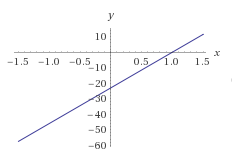
\includegraphics[width=7cm]{allg/funktionen/img/FunktionsplotAusGleichung.png}}}
\noTRAINER{\raisebox{-1cm}{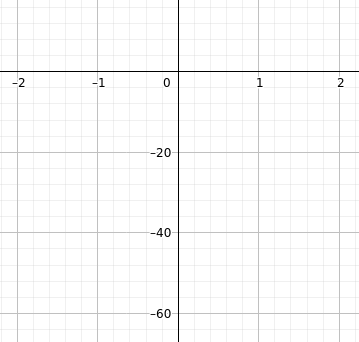
\includegraphics[width=7cm]{allg/funktionen/img/KoordSystemFaktor20.png}}}


Die Lösung obiger Gleichung kann nun auf der $x$-Achse ungefähr bei $x=1.0$ abgelesen werden.

\TALSAadBMTA{171ff}{601. a) b) c) e) f) 602. b) c) d) 603. b) c)
 604. 605. a) c) e) 606. a) c) 607. c) d) g) 608. a) 609. a) 610. a)
 611. a) 613. a) 616. c) 622. Flächen: 626. 628. und 629.}
\GESOAadBMTA{252ff}{30. Tropfsteinhöle visualisieren}
\GESO{\newpage}


\GESO{\subsection{Aus alten Maturaprüfungen}

\subsubsection{Serie 2017 Aufgabe 10}

Gegeben ist folgende Funktionsgleichung der Geraden $g$:

$$g: y = -3.75x + \frac{1}{4}$$

a) Bestimmen Sie die Schnittpunkte von $g$ mit den Koordinatenachsen.
Geben Sie die exakten Werte an.

\TNT{7.2}{Schnittpunkt mit der $y$-Achse heißt $x=0$ also $y=-3.75\cdot{}0 + \frac{1}{4} = \frac{1}{4}$. Somit ist der Schnittpunkt mit der $y$-Achse $(0 | \frac{1}{4})$.

Schnittpunkt mit der $x$-Achse heißt $y=0$ also $0=-3.75\cdot{}x + \frac{1}{4}$. Gleichung Auf"|lösen: Auf beiden Seiten $- \frac{1}{4}$ ergibt

$$-\frac{1}{4} = -3.75 x$$
Nun beide Seiten dividieren durch $-\frac{1}{4}$ ergibt:

$$1 = 15x$$

Und somit ist $x=\frac{1}{15}$, und der gesuchte Punkt auf der $x$-Achse lautet $(\frac{1}{15} | 0)$.


}%% END 'noTRAINER'
\newpage

b) Nennen Sie zwei verschiedene Punkte $A(x_A | y_A)$ und $B(x_B | y_B)$, die
auf $g$ liegen und folgende Vorgabe erfüllen:

$x_A$, $y_A$, $x_B$ und $y_B$ müssen ganzzahlig sein. \TRAINER{\zB Wertetabelle im TR mit x= -10 step 1}

\TNT{16}{
  \bbwGraph{-4}{4}{-13}{6}{
    \bbwFunc{-3.75*\x+0.25}{-2:3.5}
 \bbwDot{3,-11}{blue}{west}{B}
 \bbwDot{-1,4}{blue}{east}{A}
}%% END BBW Graph
}%% END TRAINER
\newpage



\subsubsection{2016 Aufgabe 7}

Carunternehmen A bietet folgenden Tarif an:
Pro Tag CHF 300.-- Grundtaxe und für jeden gefahrenen Kilometer CHF 1.50.

Bei Unternehmen B bezahlte eine Reisegruppe für Grund- und Kilometertaxe für einen
Tagesausflug von 600 km den Betrag von CHF 1320.--.

Eine andere Gruppe, die ebenfalls mit Unternehmen B fuhr, bezahlte mit demselben
Tarif für einen Tagesausflug von 750 km den Betrag von CHF 1590.-- .

a) Bestimmen Sie die Kostenfunktionen $y = f(x)$ für die Unternehmen A und B;
$x$ = Anzahl km gefahrene Strecke, $y$ = Anzahl CHF Gesamtkosten.

\TNT{5.6}{A: $y=1.5x + 300$

B: Steigungsdreieck: $a=\frac{1590 - 1320}{750-600} = \frac{270}{150} = 1.8$ daraus folgt $y = 1.8x + b$. Nun können wir die erste Reisegruppe einsetzen: $1320 = 1.8\cdot{}600 + b$ und somit ist $b= 240$. Die Funktionsgleichung lautet also

B: $y = 1.8x + 240$
\vspace{30mm}
}%% END TRAINER

b)  Bei welcher Fahrstrecke sind beide Firmen\footnote{Müsste in der Aufgabenstellung wohl «Unternehmen» lauten; wird aber vorausgesetzt, dass verstanden wird, was gemeint ist.} gleich teuer?

\TNT{5.6}{
$y$ = Kosten gleichsetzen: $1.5x + 300 = 1.8x + 240$. Gleichung auf"|lösen: $60 = 0.3x$ und somit $x=200$. Ergo: Bei 200 km sind beide Unternehmen (=Firmen) gleich teuer.
}%% end TRAINER
\newpage



c) 
Zwei weitere Firmen, C und D, haben folgende Kostenfunktion:

Firma C: $y = 1.8x + 250$ , Firma D: $y = 2.5x + 150$ ;

$x$ = Anzahl km gefahrene Strecke, $y$ = Anzahl CHF Gesamtkosten.

Eine Reisegruppe wählt für einen Tagesausflug von 300 km Länge Firma D, da diese
den ansprechenderen Internetauftritt hat. Um welchen Betrag wird diese Reise gegen-
über dem Angebot von Firma C teurer?

\TNT{4}{300 km in beide Funktionsgleichungen als $x$-Wert eintragen: C kostet $1.8\cdot{}300 + 250 = 790$; D kostet $2.5\cdot{}300 + 150 = 900$. Somit kostet D CHF 110.-- mehr als C.

}%% end TRAINER
\newpage


\subsubsection{2018 Serie 1 Aufgabe 9}

Gegeben ist die Gerade $g$ mit der Funktionsgleichung $y = \frac{2}{3}x-4$.

a) Berechnen Sie den Schnittpunkt von $g$ mit der $x$-Achse.

\TNT{4}{Schnittpunkt mit der $x$-Achse heißt $y=0$. Somit $0 = \frac{2}{3}x - 4$ nach $x$ auf"|lösen:
$4=\frac{2}{3}x$ $\longrightarrow$ $6 = x$. Der Schnittpunkt ist folglich $(6|0)$.

  \vspace{30mm}
}%% end TRAINER

b) Welche der folgenden Punkte $A$, $B$, $C$ liegen \textit{oberhalb}, welche
\textit{unterhalb} und welche \textit{auf} der Geraden $g$?

$$A\left(5\middle|-\frac{3}{4}\right), B(2.1|-2.6), C(50|30)$$

\textbf{Antworten:}

\begin{tabular}{lcl}
$A$ liegt & \TRAINER{unterhalb}\noTRAINER{....................................................} & der Geraden $g$.\\
$B$ liegt & \TRAINER{auf}\noTRAINER{....................................................} & der Geraden $g$.\\
$C$ liegt & \TRAINER{oberhalb}\noTRAINER{....................................................} & der Geraden $g$.\\

 \end{tabular}{

\TNT{5.2}{Jeweils $x$ in die Gleichungen einsetzen und mit $y$ vergleichen.}%% End TNT
}

